\section{Validierung anhand des Hilti Auspressgerätes}
\label{Kapitel:Auspressgeraet}
Die von Hilti hergestellten chemischen Dübelmassen bestehen aus zwei Komponenten. Diese werden bei der Anwendung gemischt und in ein vorgebohrtes Loch gedrückt. Durch das Mischen der Komponenten beginnt der Mörtel auszuhärten und befestigt dadurch eine ebenfalls in das Loch eingeführte Gewindestange.

Die Mörtelkomponenten werden mit einem eigens dafür entwickelten Auspressgerät in die Löcher gedrückt. Dieses Auspressgerät soll gleichzeitig möglichst zuverlässig und stabil sein, aber auch so konstruiert, dass für die Anwendung wenig Kraft gebraucht wird und exakt so viel Fluid ausgepresst wird wie vom Anwender gewollt.
Das derzeit auf dem Markt erhältliche Gerät ist in Abbildung~\ref{fig:Auspressgeraet} gezeigt.
%
\begin{figure}[b]
    \centering
    \subfloat[Handgerät]{
        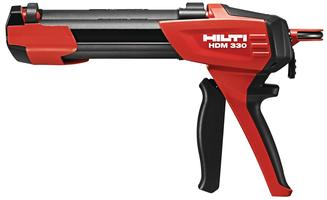
\includegraphics[width=0.31\textwidth]{figures/Auspressgeraet.jpg}
        \label{fig:Auspressgeraet:subA}
    }
    \subfloat[Akkugerät]{
        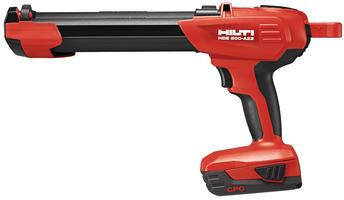
\includegraphics[width=0.31\textwidth]{figures/AuspressgeraetAkku.jpg}
        \label{fig:Auspressgeraet:subB}
    } 
    \subfloat[Mörtel Kasette]{
        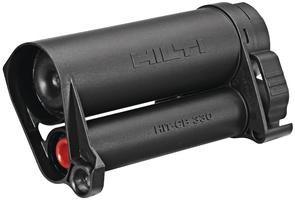
\includegraphics[width=0.31\textwidth]{figures/AuspressgeraetKasette.jpg}
        \label{fig:Auspressgeraet:subC}
    }
    \caption{Geräte zum Auspressen von Hilti Injektionsmörtel.\\In \subref{fig:Auspressgeraet:subA} ist das Handgerät zu sehen, in \subref{fig:Auspressgeraet:subB} die Ausführung mit Akku, bei der das Auspressen auf Knopfdruck geschieht.
    In \subref{fig:Auspressgeraet:subC} ist eine Kasette abgebildet, in die die Mörtelbeutel gelegt werden.}
    \label{fig:Auspressgeraet}
\end{figure}
%
Das Mischen der beiden Komponenten geschieht in einem Mischer, der vorne auf das Auspressgerät aufgeschraubt wird (Abbildung~\ref{fig:Mischer}).
%
\begin{figure}
    \centering
    \subfloat[Mischeraufsatz]{
    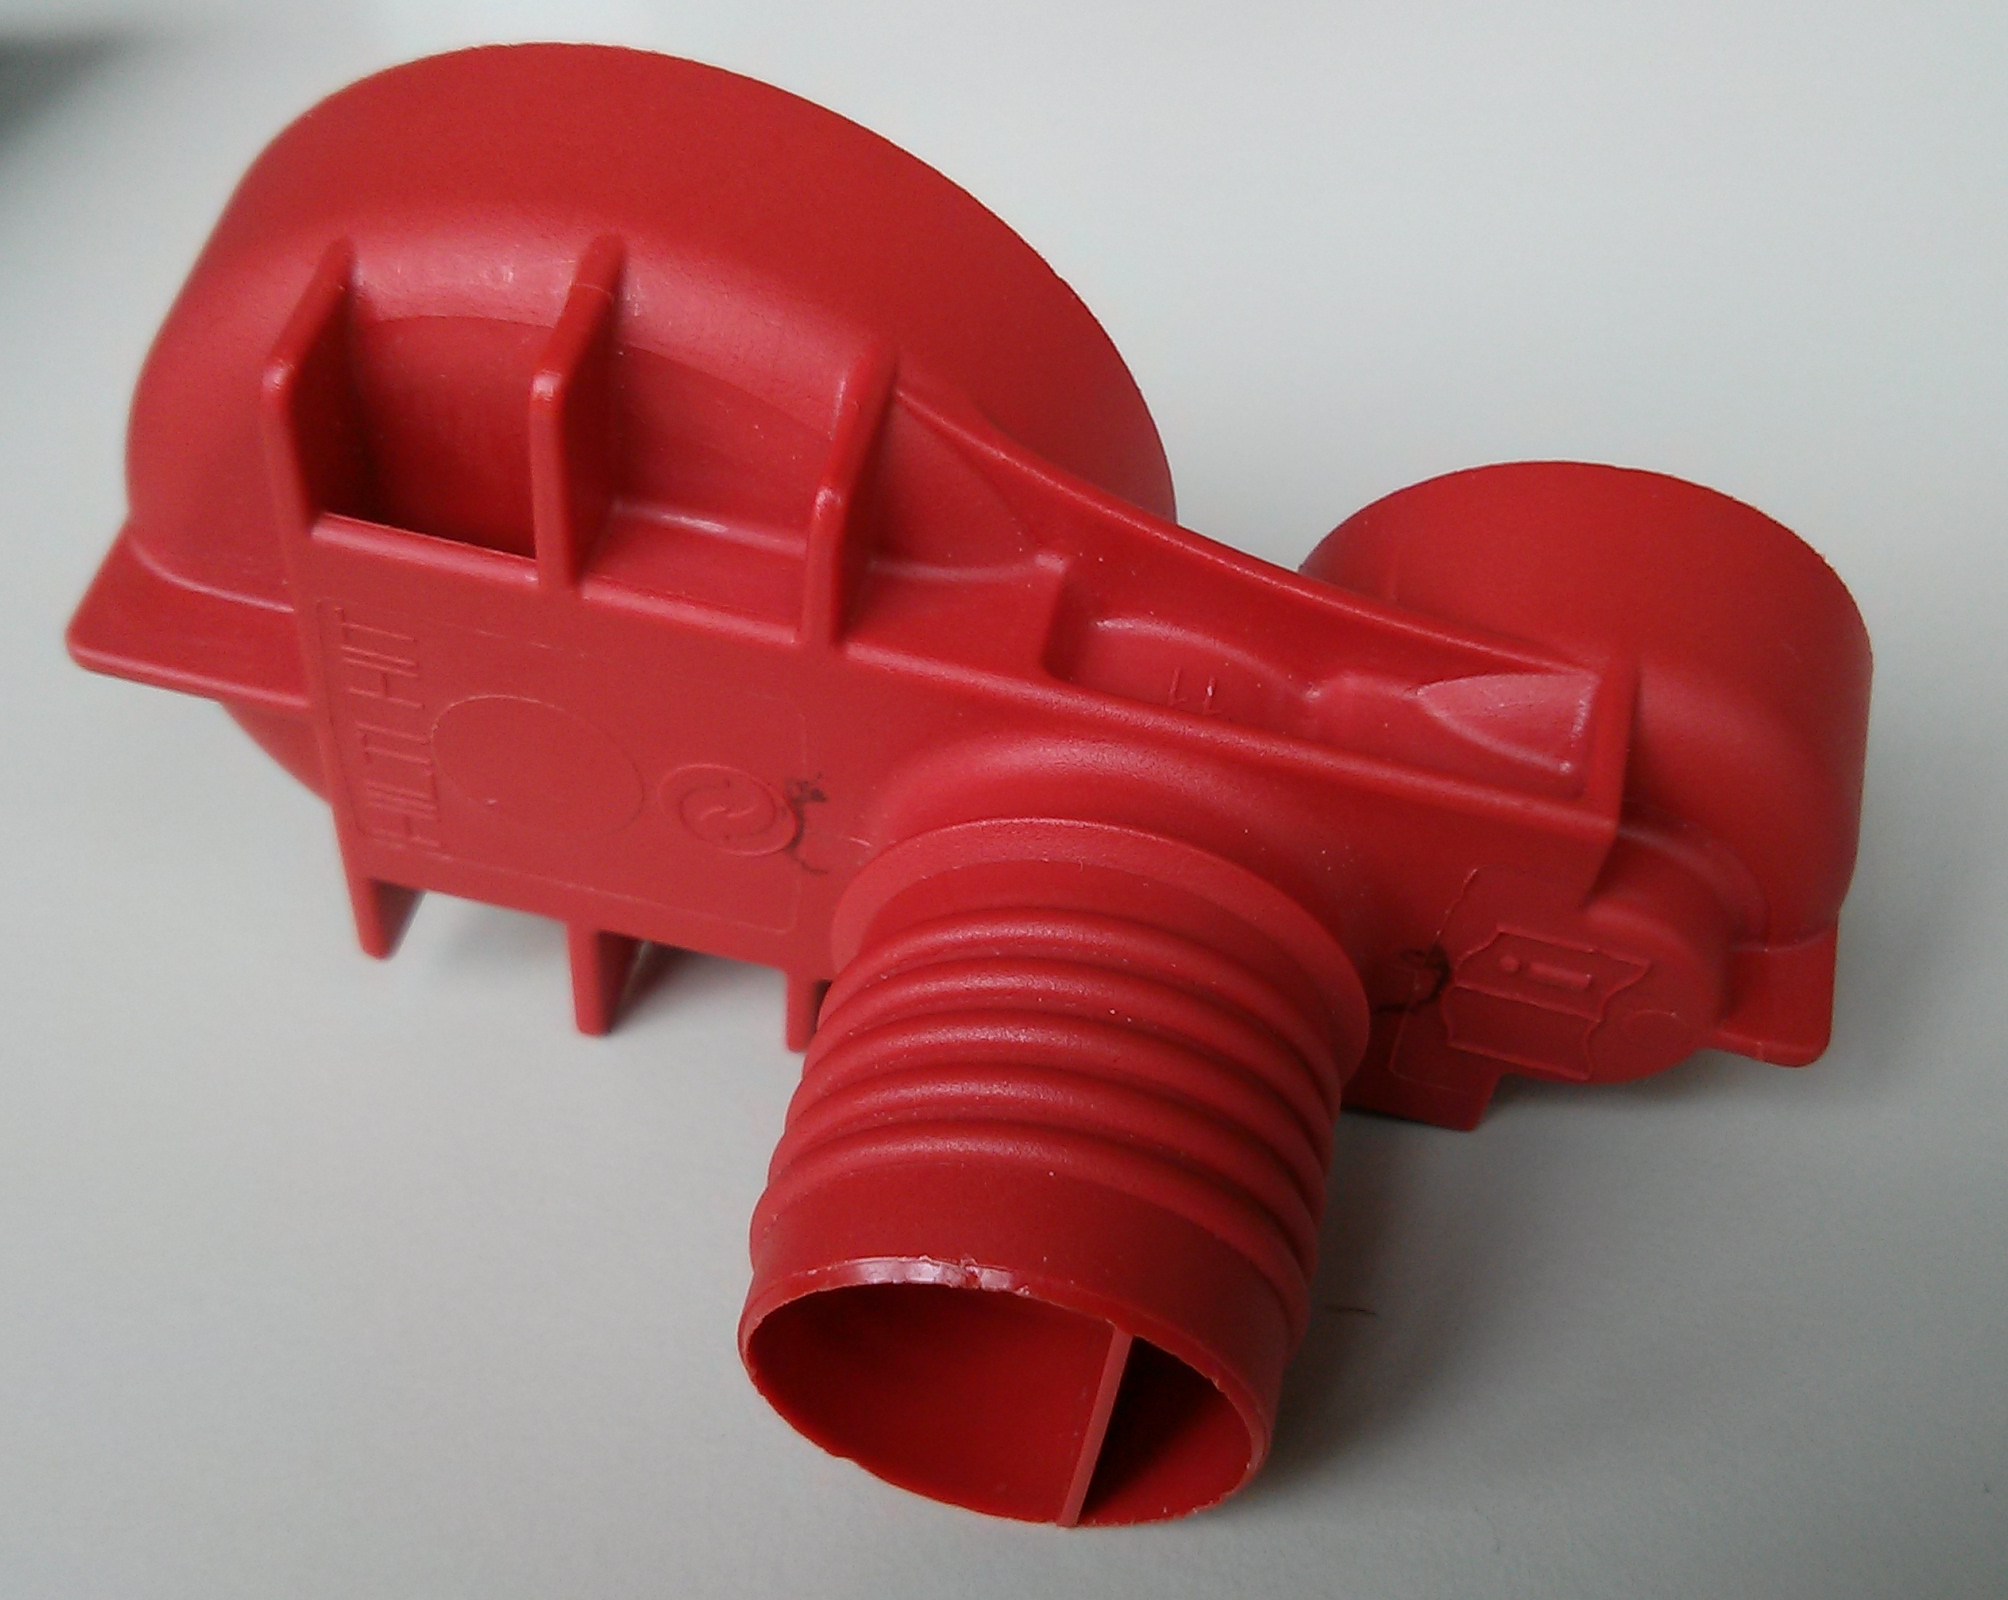
\includegraphics[width=0.2\textwidth]{figures/Mischeraufsatz.png}
        \label{fig:Mischer:subA}
    }
    \subfloat[Mischer HIT-RE-M]{
    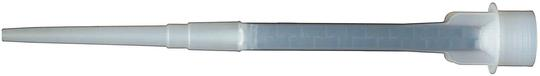
\includegraphics[width=0.67\textwidth]{figures/Mischer.jpg}
        \label{fig:Mischer:subB}
    }
    \caption{Das Mischermodell HIT-RE-M, in dem die Mörtelkomponenten beim Auspressen gemischt werden.}
    \label{fig:Mischer}
\end{figure}
%
Dieser Mischer kann jeweils nur einmal verwendet werden, weil der Mörtel ab dem Zeitpunkt des Mischens beginnt auszuhärten und so den Mischer verstopft, sobald das Auspressen gestoppt wird. Es ist deshalb im Interesse des Verbrauchers, dass der Mischer im Erwerb sehr preiswert ist. Trotzdem soll er die Komponenten zuverlässig mischen, da dies entscheidend ist für die maximale Zuglast der Dübel.

Diese Ansprüche an das Gerät und den Mischer erfordern ein hohes Mass an Verständnis für die Vorgänge wäh"-rend des Auspressens. Daher ist die Vermessung, Simulation und Verbesserung des Gesamtsystems ein Forschungsthema der Hilti AG.
%
\subsection{Messaufbau}
Das für die Mörtel verwendete Auspressgerät besteht zum grössten Teil aus Kunststoff. Da dieses selber elastische Eigenschaften besitzt, ist es sehr schwierig, die viskoelastischen Eigenschaften eines Fluides zu bestimmen, das durch das Gerät fliesst.
Um den Einfluss des Gerätes auf das Fluid auszuschliessen, wurde die Geometrie des Auspressgerätes in einer sogenannten Funktionsersatzprüfung (FEP) aus Metall nachgebaut. In Abbildung~\ref{fig:FEP} sind Aufnahmen dieser FEP zu sehen; in \ref{fig:FEP_schema} ist der Aufbau schematisch dargestellt.
%
\begin{figure}[hbt]
    \centering
    \subfloat[Metallnachbau]{
        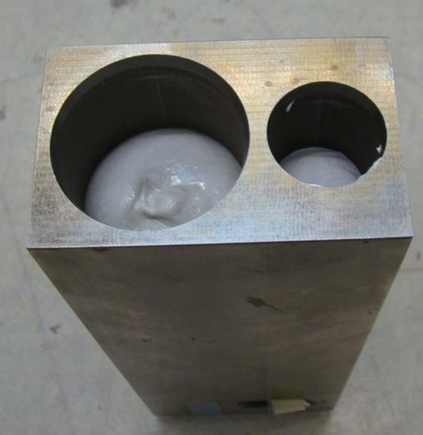
\includegraphics[height=7em]{figures/FEP_1.png}
        \label{fig:FEP:subA}
    }
    \subfloat[mit Mörtel gefüllt]{
        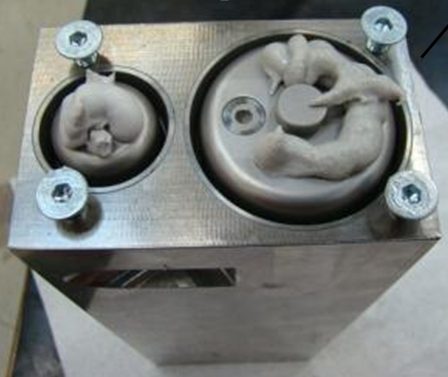
\includegraphics[height=7em]{figures/FEP_2.png}
        \label{fig:FEP:subB}
    } 
    \subfloat[Übergang zwischen Kolben und Mischer]{
        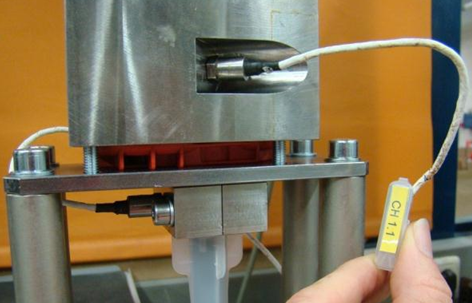
\includegraphics[height=7em]{figures/FEP_3.png}
        \label{fig:FEP:subC}
    }
    \caption{Der Messaufbau für die Funktionsersatzprüfung des Auspressgerätes.
    In Abbildung~\subref{fig:FEP:subA} ist der Nachbau der Geometrie aus Metall zu sehen, der in \subref{fig:FEP:subB} mit Mörtel befüllt worden ist.
    Dieser Mörtel wird dann von Kolben durch eine Blende in den Mischer gepresst. Die Schnittstelle zum Mischer ist in \subref{fig:FEP:subC} zu sehen.}
    \label{fig:FEP}
\end{figure}
%
\begin{figure}
    \centering
    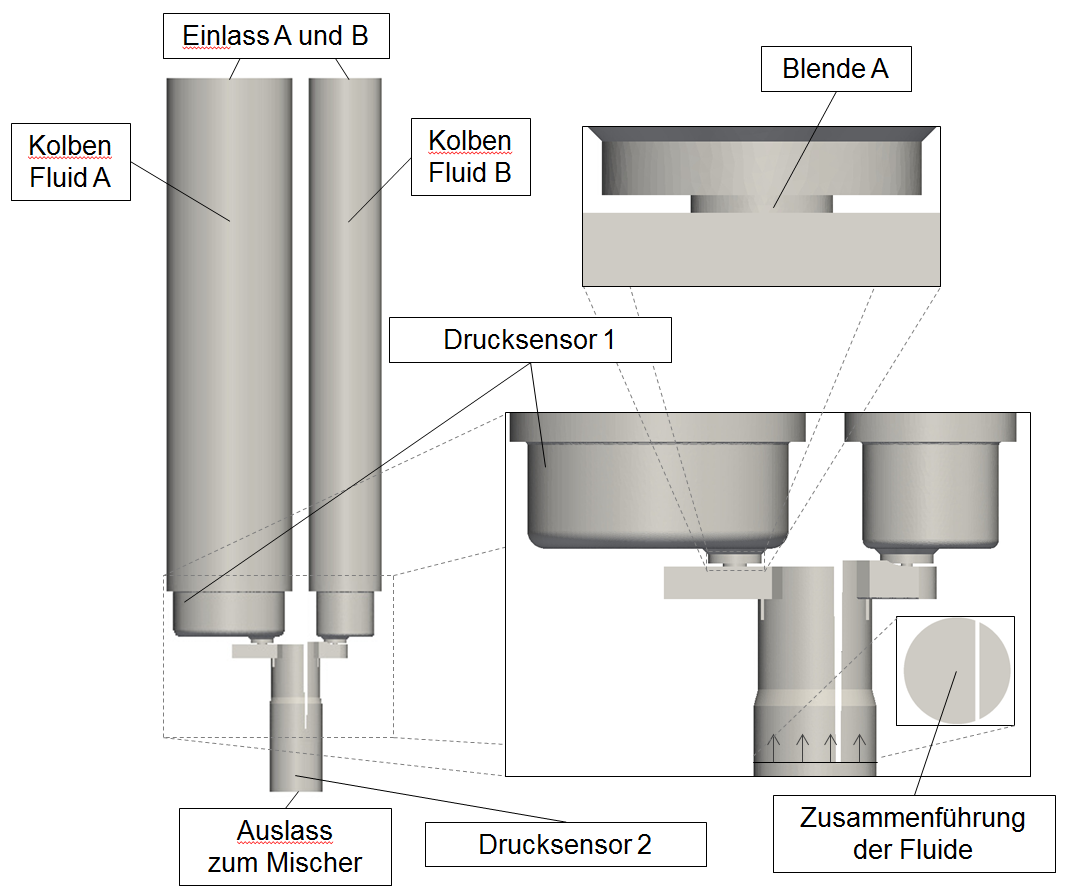
\includegraphics[width=\textwidth]{figures/FEP_Schema.png}
    \caption{Schematische Zeichnung der Funktionsersatzprüfung. Zu sehen sind die Kolbenwege der beiden Fluide,
    die Drucksensoren 1 und 2 und die Blenden, deren Durchmesser variiert werden kann. Der Drucksensor 1 kann entweder im A- oder im B-Kolben eingesetzt werden.}
    \label{fig:FEP_schema}
\end{figure}

Bei der Messung wird der Mörtel in die Metallröhren eingefüllt und dann von den Kolben nach unten gedrückt. Im Übergang zwischen FEP und Mischer ist auf jeder Seite eine auswechselbare Blende eingebaut, die den Durchmesser der engsten Stelle bestimmt, durch die das Fluid fliessen muss. Danach kommen die beiden Ströme zusammen und werden in den Mischer geleitet.

Die variablen Grössen bei der Versuchsausführung sind dabei die Kolbengeschwindigkeit (und damit der Volumenstrom), die Grösse der eingelegten Blenden und der Typ des verwendeten Mörtels. In der Praxis sind dabei auf den zwei Seiten jeweils die A und die B Komponente des Mörtels.
In der FEP wurden beide Seiten mit derselben Mörtelkomponente befüllt. Der Grund war die Vergleichbarkeit mit der Simulation, bei der auf eine Mehrkomponentensimulation mit unterschiedlichen Materialgesetzen verzichtet werden sollte.
%, um den Vergleich mit den Simulationen einfach zu machen, jeweils nur ein Typ Mörtel eingesetzt.

Der Druck wird jeweils vor dem Durchströmen der Blende und vor dem Mischereingang (Drucksensor 1 und 2 in Abbildung~\ref{fig:FEP_schema}) gemessen. Das Messergebnis ist der Druckunterschied zum Umgebungsdruck.
Dabei kann Drucksensor 1 entweder auf der A- oder auf der B-Seite eingesetzt werden und damit den Druckverlust über die A- oder die B-Blende messen.
Desweiteren wurde die Kraft, die für das Runterdrücken der Kolben notwendig ist, gemessen.
%
\subsection{Simulation}
Durch den Vergleich der durchgeführten Messungen mit Simulationen sollen Aussagen über die Verlässlichkeit der verwendeten Modelle gewonnen werden können.
Dazu wurde die Geometrie der FEP und des Mischers in CAD Programmen modelliert und mit Ansys ICEM vernetzt. Verwendet wurde ein Tetraedernetz mit ca. \num{3e6} Zellen. Dabei wurde darauf geachtet, dass die kritischen Regionen, wie zum Beispiel die Blende in der FEP, besonders fein vernetzt sind, wäh"-rend Regionen in denen keine grosse Veränderungen in den Variablen zu erwarten sind, gröber vernetzt wurden. Beispiele sind in den Abbildungen~\ref{fig:FEP_Gitter} und \ref{fig:Mischer_Gitter} zu sehen.

%Aufgrund der variablen Viskosität mussten die viskoelastischen Simulationen mit sehr kleinen Zeitschritten gerechnet werden. Wegen der resultierenden langen Rechenzeit
%wurden für das Auspressgerät nur die scherratenabhängigen Modelle verwendet und keine viskoelastischen Simulationen durchgeführt.
%
\begin{figure}
    \centering
    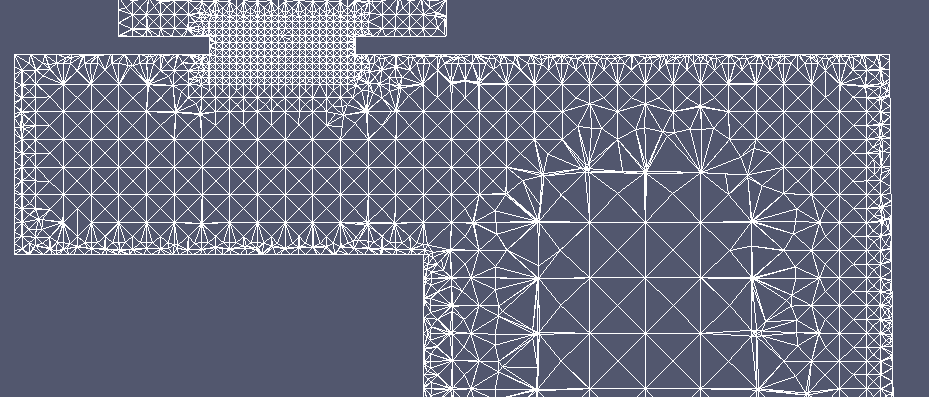
\includegraphics[width=\textwidth]{figures/FEP_Gitter1.PNG}
    \caption{Ein Ausschnitt des verwendeten Gitters für die FEP.
    Zu sehen ist oben links die Blende, die sehr fein aufgelöst ist. Nach unten wird das Netz wieder gröber, da die erwarteten Änderungen in $\u$ und $p$ kleiner sind.}
    \label{fig:FEP_Gitter}
\end{figure}
%
\begin{figure}
    \centering
    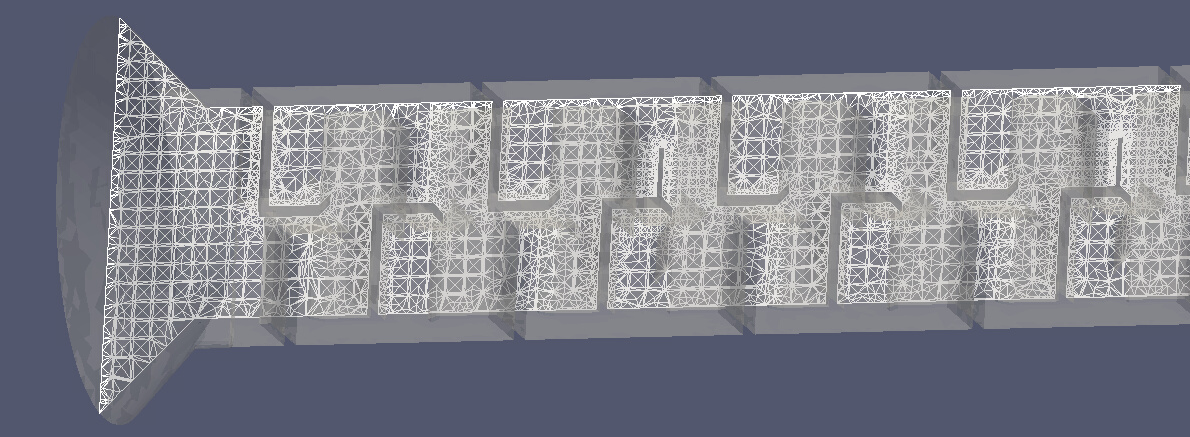
\includegraphics[width=\textwidth]{figures/Mischer_Gitter1.PNG}
    \caption{Ein Ausschnitt des verwendeten Gitters für den Mischer.
    Die Geometrie ist dabei transparent hellgrau dargestellt um den Ort des gezeigten Schnittes durch das Netz zu verdeutlichen.}
    \label{fig:Mischer_Gitter}
\end{figure}
%

Simuliert wurde mit dem Löser \codeemph{simpleFoam}. Dabei wurde stets eine stationäre Lösung angestrebt, bei der die Geschwindigkeit an den Einlässen vorgegeben und dann gerechnet wurde, bis sich ein konstanter Gegendruck ausgebildet hatte. Das setzt voraus, dass der Einfluss des Kolbens mit einer konstanten Anströmung gleichgesetzt werden kann, was natürlich nur bei ausreichendem Abstand zwischen Kolben und Blende hinreichend genau stimmt.

Die berechneten Felder waren die Geschwindigkeit $\u$ und der Druck $p$. Als Randbedingung wurde für $\u$ beim Einlass ein konstanter Wert, beim Auslass ein Null-Gradient und an den Wänden eine Haftbedingung vorgegeben. Der Druck $p$ wurde am Einlass auf Null gesetzt und an allen anderen Rändern ein Null-Gradient vorgegeben.
Für die Startlösung wurden, wann immer möglich, die Werte einer früheren Rechnung verwendet. Dadurch kann die Konvergenz drastisch beschleunigt werden. 
Falls für ein Netz keine alte Startwerte existierten, wurden alle Werte von $p$ und $\u$ im Inneren mit Null initialisiert. Das ist vor allem für den Mischer eine äusserst ungünstige Anfangsbedingung. In diesen Fällen konnte Konvergenz nur erreicht werden, wenn die Relaxationsparameter hinreichend klein gewählt wurden.
Die Viskosität $\eta$ ist direkt abhängig von $\u$ und musste deshalb bei Start- oder Randbedingungen nicht berücksichtigt werden.
%
\subsection{Ergebnisse}
Für die Validierung der Simulationen standen Messungen mit un"-ter"-schiedli"-chen Mörteln, Kolbengeschwindigkeiten und Blendendurchmessern bei der FEP zur Verfügung. Da bei der Messung am Auslass der FEP ein Mischer montiert wurde, konnte mit einer Messung an den beiden Druckaufnehmern jeweils gleich der Druckverlust über die Blende und der Druckverlust im Mischer gemessen werden.

In den Simulationen wurden der Mischer und die FEP separat behandelt, da dadurch die Konvergenz beschleunigt werden konnte. Eine Kontroll"-si"-mulation mit einer kompletten Geometrie von FEP und Mischer hat ergeben, dass dadurch keine Einbussen bei der Genauigkeit entstehen.


\subsubsection{Funktionsersatzprüfung}
Bei der FEP wurden acht Messungen, mit je zwei Mörteln, zwei Kolben"-ge"-schwindig"-kei"-ten und zwei Blendenkonfigurationen durchgeführt. 
Eine Bei"-spiel"-kon"-fi"-gura"-tion mit Blendendurchmesser $\emptyset_A=10$ mm und $\emptyset_B=4$ mm ist in Abbildung~\ref{fig:fepSimResult} zu sehen.
In Tabelle~\ref{fig:fepVergleich} sind die gemessenen und die simulierten Druck"-verluste über die Blende aufgeführt. Simulationen wurden mit den rein scherratenabhängigen Modellen durchgeführt. 
Der Druckverlust wurde dabei jeweils auf der Seite gemessen, die der eingefüllten Mörtelkomponente entspricht.
Das bedeutet, dass für die A Komponente die Messstelle auf der A Seite in Abbildung~\ref{fig:FEP_schema} verwendet wurde.
%
\begin{table}[tb]
\noindent\makebox[\textwidth]{%
    \begin{tabular}{l c c c r r r} 
        \toprule[1.5pt]
        \multicolumn{4}{c}{\textbf{Messaufbau}} &
        \multicolumn{2}{c}{\textbf{Druckverlust}} &
        \textbf{Fehler}\\
        \textbf{Mörtel} & \textbf{Blende A}& \textbf{Blende B} & $\u$
        & \textbf{Messung }& \textbf{Simulation} & \\
        & \si{mm} & \si{mm} & \si{mm.s^{-1}}
        & \si{Bar}& \si{Bar} & \%\\
     \cmidrule(lr){1-4}
     \cmidrule(lr){5-6}
     \cmidrule(lr){7-7}
    \multirow{4}{*}{\moertelA{} A} &  \multirow{2}{*}{4} & \multirow{2}{*}{2} & 2.1 & 0.3 & 0.38  & 28\\
                                                    %\cline{4-7}
                              &                     &                    & 4   & 0.43 & 0.5  & 17\\
                              %\cline{2-7}
                              \addlinespace
                              & \multirow{2}{*}{10} & \multirow{2}{*}{4} & 2.1 & 0.28 & 0.23 & 16\\
                                                    %\cline{4-7}
                              &                     &                    & 4   & 0.32 & 0.29 &  10\\
     \cmidrule(lr){2-4}
     \cmidrule(lr){5-6}
     \cmidrule(lr){7-7}
    \multirow{4}{*}{\moertelA{} B} &  \multirow{2}{*}{4} & \multirow{2}{*}{2} & 2.1 & 0.77 & 0.38 & 51\\
                                                    %\cline{4-7}
                              &                     &                    & 4   & 0.89 & 0.45 & 50\\
                              %\cline{2-7}
                              \addlinespace
                              & \multirow{2}{*}{10} & \multirow{2}{*}{4} & 2.1 & 0.53 & 0.29 & 45\\
                                                    %\cline{4-7}
                              &                     &                    & 4   & 0.58 & 0.33 & 42\\
     \cmidrule(lr){2-4}
     \cmidrule(lr){5-6}
     \cmidrule(lr){7-7}
    \multirow{4}{*}{\moertelB{} A} &  \multirow{2}{*}{4} & \multirow{2}{*}{2}  & 2.1 & 0.37 & 0.26 &31\\
                                                    %\cline{4-7}
                              &                     &                    & 4   & 0.48 & 0.35 &26\\
                              %\cline{2-7}
                              \addlinespace
                              & \multirow{2}{*}{10} & \multirow{2}{*}{4} & 2.1 & 0.24 & 0.14 &40\\
                                                    %\cline{4-7}
                              &                     &                    & 4   & 0.33 & 0.18 &44\\
     \cmidrule(lr){2-4}
     \cmidrule(lr){5-6}
     \cmidrule(lr){7-7}
    \multirow{4}{*}{\moertelB{} B} &  \multirow{2}{*}{4} & \multirow{2}{*}{2}  & 2.1 & 0.41 & 0.31 &25\\
                                                    %\cline{4-7}
                              &                     &                    & 4   & 0.51 & 0.40 &22\\
                              %\cline{2-7}
                              \addlinespace
                              & \multirow{2}{*}{10} & \multirow{2}{*}{4} & 2.1 & 0.44 & 0.21 &53\\
                                                    %\cline{4-7}
                              &                     &                    & 4   & 0.48 & 0.23 &51\\
    \bottomrule[1.5pt]
\end{tabular}}
    \caption{Die gemessenen und simulierten Konfigurationen der FEP mit den rein scherratenabhängigen Modellen. Der Druck wurde auf der Seite der entsprechenden Mörtelkomponente gemessen.}
    \label{fig:fepVergleich}
\end{table}
%
\begin{figure}[htb]
    \centering
    \rotatebox{90}{
    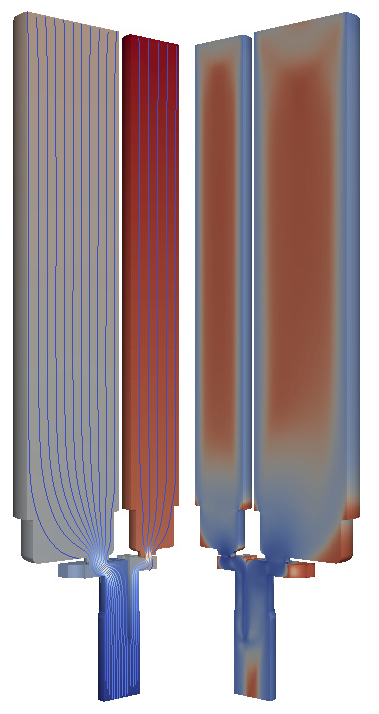
\includegraphics[width=0.5\textwidth]{figures/fepSim.PNG}
    }
    \caption{Eine Simulation der Funktionsersatzprüfung. Unten die Druckverteilung mit eingezeichneten Stromlinien, oben die variable Vikosität. Schön zu sehen ist das blockartige Strömen des Mörtels im Einlaufkolben anhand des grossen roten Gebietes hoher Viskosität und die abrupte Abnahme der Viskosität in den Blenden.}
    \label{fig:fepSimResult}
\end{figure}

Die simulierten Widerstände sind in der Tendenz konsistent mit der Messung. Die absoluten Werte zeigen jedoch eine Abweichung von bis zu 50\%. Dies zeigt, dass die verwendeten Modelle und Parameter noch nicht vollständig in der Lage sind, die Realität zu simulieren. So liegen die Scherraten, die in der engen \SI{2}{mm} Blende auftreten, in einem Bereich der im Kapillarrheometer nicht mehr auftritt. In diesem Bereich wird also das Modell extrapoliert.
Allerdings ist es möglich, dass ein Teil der Abweichung auf die Messungenauigkeit der Messgeräte zurückgeführt werden kann. 
Bei den Messstellen wird jeweils der Unterschied zum Umgebungsdruck gemessen. Die Messgeräte besitzen eine Toleranz von 1-3\%. 
Bei der Berechnung der Druckdifferenz, die Betragsmässig viel kleiner ist als die Messwerte, verstärkt sich diese Unsicherheit und kann bis zu 40\% betragen.
%
\subsubsection{Mischer}
Da beim Mischer keine Blenden eingelegt werden, gibt es nur noch 8 statt 16 verschiedene Konfigurationen. Diese bestehen aus je einem von vier Mörteln und einer von zwei Einlassgeschwindigkeiten.
Die Einlass"-ge"-schwin"-dig"-keit bei der Messung wird bestimmt durch die Kolbengeschwindigkeit der FEP, da die Systeme gekoppelt sind. Für die Simulation wurde der entsprechende Volumenstrom bei der FEP genommen und daraus die Einlassgeschwindigkeit bestimmt, da der Mörtel als inkompressibel behandelt wird.
\begin{equation}
    \u_{\text{\tiny Mischer}} = \frac{R_A^2+R_B^2}{R_M^2} \cdot \u_{\text{\tiny FEP}} = 8.5 \cdot \u_{\text{\tiny FEP}}~,
\end{equation}
wobei $R_A$, $R_B$ und $R_M$ die Radien der Einlässe des A- und B-Kolbens und des Mischers sind.
In Tabelle~\ref{fig:mischerVergleich} sind die gemessenen und die simulierten Druckverluste über den Mischer aufgeführt, in Abbildung~\ref{fig:mischerSimResult} ist eine Beispielsimulation zu sehen.
%
\begin{table}[tb]
\noindent\makebox[\textwidth]\\
    \cmidrule(lr){1-2}
    \cmidrule(lr){3-4}
    \cmidrule(lr){5-5}
    \multirow{2}{*}{\moertelA{} A}  & 2.1 & 4.48 & 4.26 & 5\\
                               %\cline{2-5}
                               & 4   & 6.86 & 6.09 &11\\
    %\cmidrule(lr){1-2}
    %\cmidrule(lr){3-4}
    %\cmidrule(lr){5-5}
    \addlinespace
    \multirow{2}{*}{\moertelA{} B}  & 2.1 & 1.60 & 1.95 &22\\
                               %\cline{2-5}
                               & 4   & 2.16 & 2.48 &15\\
    %\cmidrule(lr){1-2}
    %\cmidrule(lr){3-4}
    %\cmidrule(lr){5-5}
    \addlinespace
    \multirow{2}{*}{\moertelB{} A}   & 2.1 & 2.43 & 2.98 &23\\
                               %\cline{2-5}
                               & 4   & 3.95 & 4.49 &14\\
    %\cmidrule(lr){1-2}
    %\cmidrule(lr){3-4}
    %\cmidrule(lr){5-5}
    \addlinespace
    \multirow{2}{*}{\moertelB{} B}   & 2.1 & 1.20 & 1.49 &24\\
                               %\cline{2-5}
                               & 4   & 1.84 & 2.13 &16\\
    \bottomrule[1.5pt]
\end{tabular}}
    \caption{Die gemessenen und simulierten Konfigurationen des Mischers mit den rein scherratenabhängigen Modellen. Die angegebene Einlassgeschwindigkeit entspricht dabei der Kolbengeschwindigkeit in der FEP.}
    \label{fig:mischerVergleich}
\end{table}
%
\begin{figure}[htb]
    \centering
    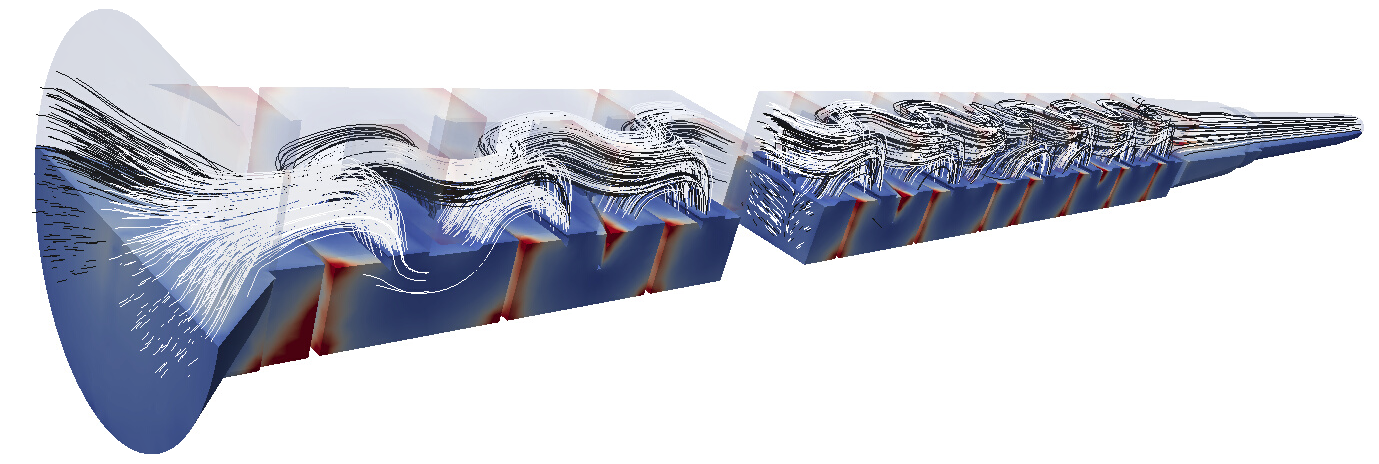
\includegraphics[width=\textwidth]{figures/MischerSimResult.png}
    \caption{Eine Simulation des statischen Mischers des Hilti Auspressgerätes. Die Viskosität in den schwach gescherten Gebieten ist deutlich höher (rot) als in den stark gescherten (blau). Die grünen und schwarzen Stromlinien sollen den Mischvorgang der beiden Mörtel-Komponenten verdeutlichen.}
    \label{fig:mischerSimResult}
\end{figure}
%
Die Abweichungen bei der Simulation des Mi\-schers sind, relativ gesehen, deutlich geringer als beim Druckverlust über die Blen\-den in der FEP. Einer der Gründe dafür ist, dass die Scherraten nun in einem Bereich sind, der auch vermessen wurden. 
Zudem ist die Messunsicherheit bei diesen Messungen deutlich geringer.
